\chapter{Частотная и фазовая модуляция}
\section{Постановка задачи}
\begin{enumerate}
\item 
Сгенерировать однотональный сигнал низкой частоты.
\item
Выполнитьфазовую модуляцию/демодуляцию сигнала по закону $u(t)=(U_m\cos(\omega t=ks(t))$ , используя встроенную функцию MatLab pmmod, pmdemod.
\item
Получить спектр модулированного сигнала.
\item
Выполнить частотную модуляцию/демодуляцию по закону 
\begin{equation}
u(t)=U_m\cos (\omega _0 t+k \int_0^t s(t)dt=\phi _0)
\end{equation}
используя встроенные функции Matlab fmmod, fmdemod.
\end{enumerate}
\section{Теоретическая часть}
Частотная модуляция — вид аналоговой модуляции, при котором информационный сигнал управляет частотой несущего колебания. По сравнению с амплитудной модуляцией здесь амплитуда остаётся постоянной.

Фазовая модуляция — один из видов модуляции колебаний, при которой фаза несущего колебания управляется информационным сигналом. Фазомодулированный сигнал s(t) имеет следующий вид:
\begin{equation} 
s(t) = g(t) \sin[2 \pi f_c t + \varphi(t)] ,
\end{equation}
где $g(t)$ — огибающая сигнала; $\phi(t)$ является модулирующим сигналом; $f_c$ — частота несущего сигнала; t — время.\\
По характеристикам фазовая модуляция близка к частотной модуляции. В случае синусоидального модулирующего (информационного) сигнала, результаты частотной и фазовой модуляции совпадают.
\section{Ход работы}
\subsection{Код Matlab}
\begin{lstlisting}
x = 0:0.01:2;
u = cos(2*pi*x);

figure;
subplot(3,1,1);
plot(x,u);
grid;
am = fmmod(u,2,30,1);
subplot(3,1,2);
plot(x,am);
grid;
modulatedSpectr = fft(am,512);
normSpectrum = modulatedSpectr.*conj(modulatedSpectr)/512;
f = 100*(-256:255)/512;
subplot(3,1,3);
plot(f,normSpectrum);
grid;
axis([min(f) max(f) 0 max(normSpectrum)]);

figure;
subplot(3,1,1);
plot(x,u);
grid;
am = pmmod(u,5,1000,pi/2);
subplot(3,1,2);
plot(x,am);
grid;
modulatedSpectr = fft(am,512);
normSpectrum = modulatedSpectr.*conj(modulatedSpectr)/512;
f = 100*(-256:255)/512;
subplot(3,1,3);
plot(f,normSpectrum);
grid;
axis([min(f) max(f) 0 max(normSpectrum)]);
\end{lstlisting}
\section{Результаты работы}


\begin{figure}[H]

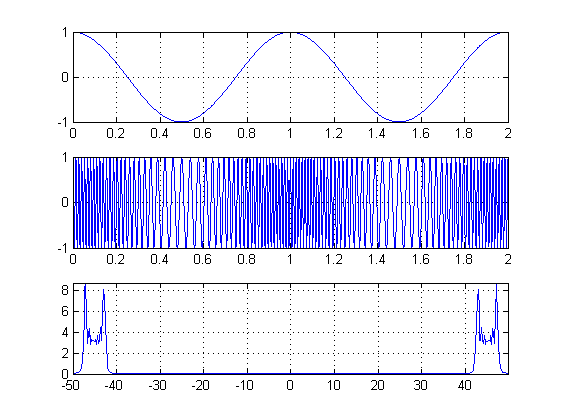
\includegraphics[width=150mm, scale = 0.9]{lab8/8_1}
   \caption{Частотная модуляция сигнала}

\end{figure}
\begin{figure}[H]

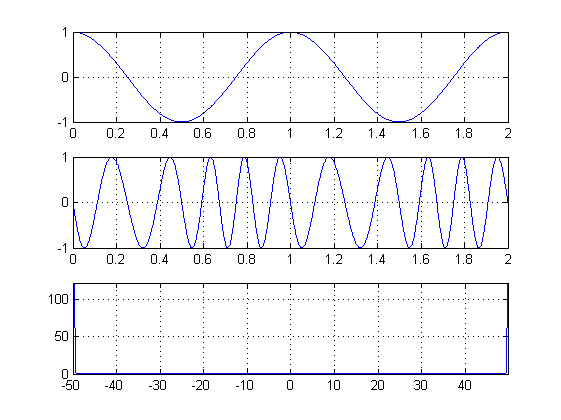
\includegraphics[width=150mm, scale = 0.9]{lab8/8_2}
   \caption{Фазовая модуляция сигнала}

\end{figure}
Смоделируем ход работы в среде Simulink:
\begin{figure}[H]

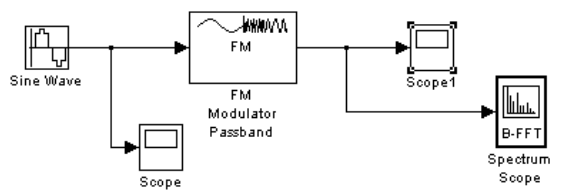
\includegraphics[width=150mm, scale = 0.9]{lab8/8_3}
   \caption{Модель для частотной модуляции}

\end{figure}
\begin{figure}[H]

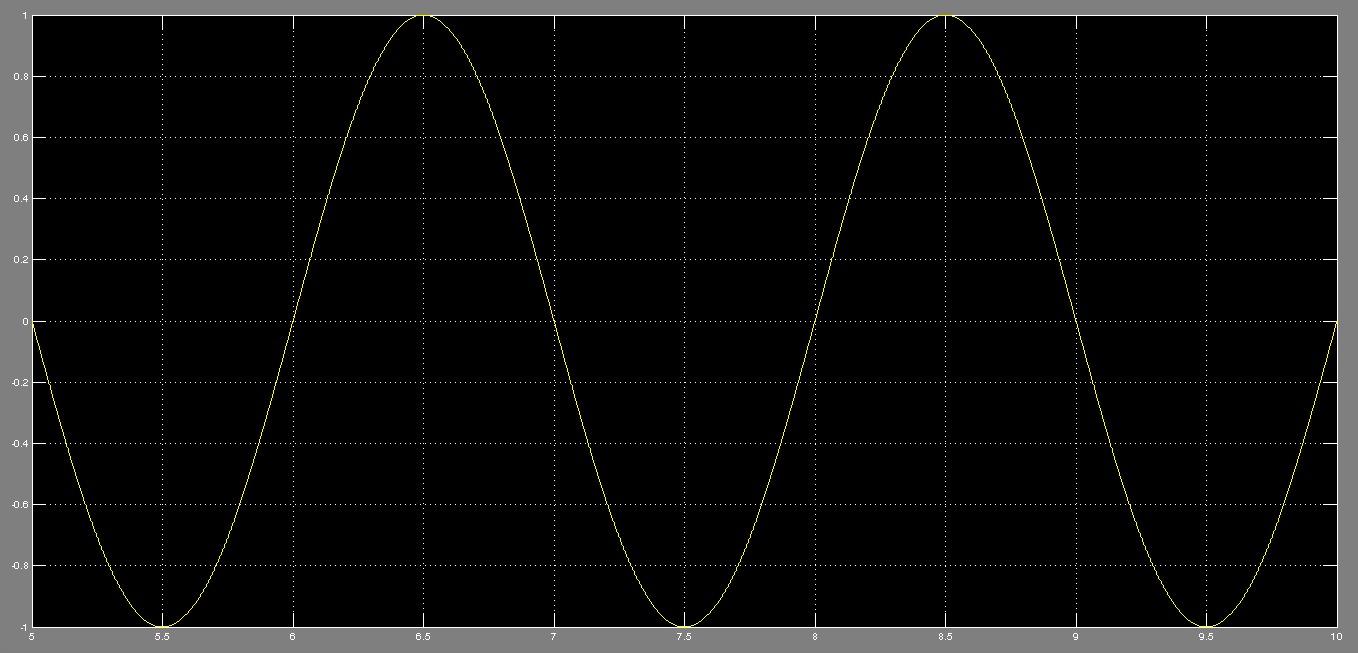
\includegraphics[width=150mm, scale = 0.9]{lab8/8_4}
   \caption{Исходный сигнал}

\end{figure}
\begin{figure}[H]

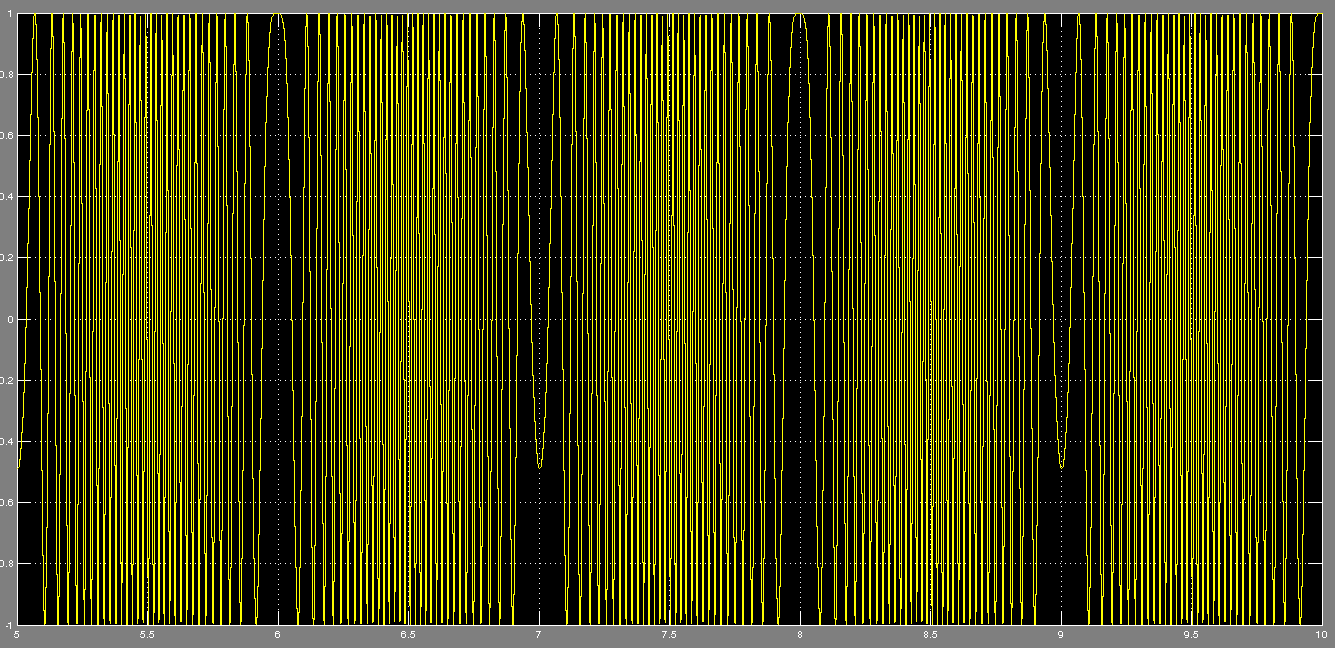
\includegraphics[width=150mm, scale = 0.9]{lab8/8_5}
   \caption{Моделированный сигнал}

\end{figure}
\begin{figure}[H]

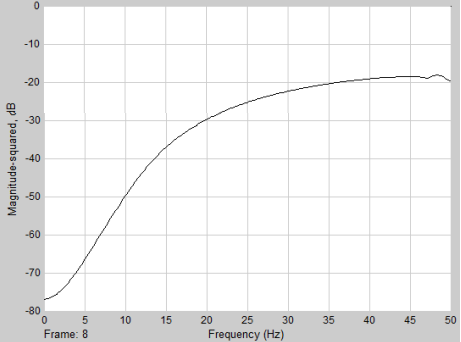
\includegraphics[width=150mm, scale = 0.9]{lab8/8_6}
   \caption{Спектр моделированного сигнала}

\end{figure}
\begin{figure}[H]

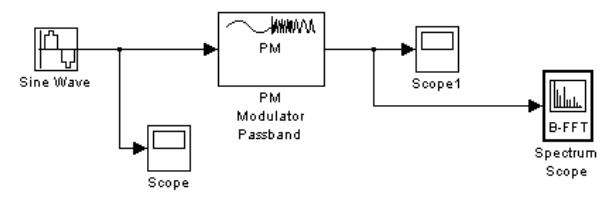
\includegraphics[width=150mm, scale = 0.9]{lab8/8_7}
   \caption{Модель для фазовой модуляции}

\end{figure}
\begin{figure}[H]

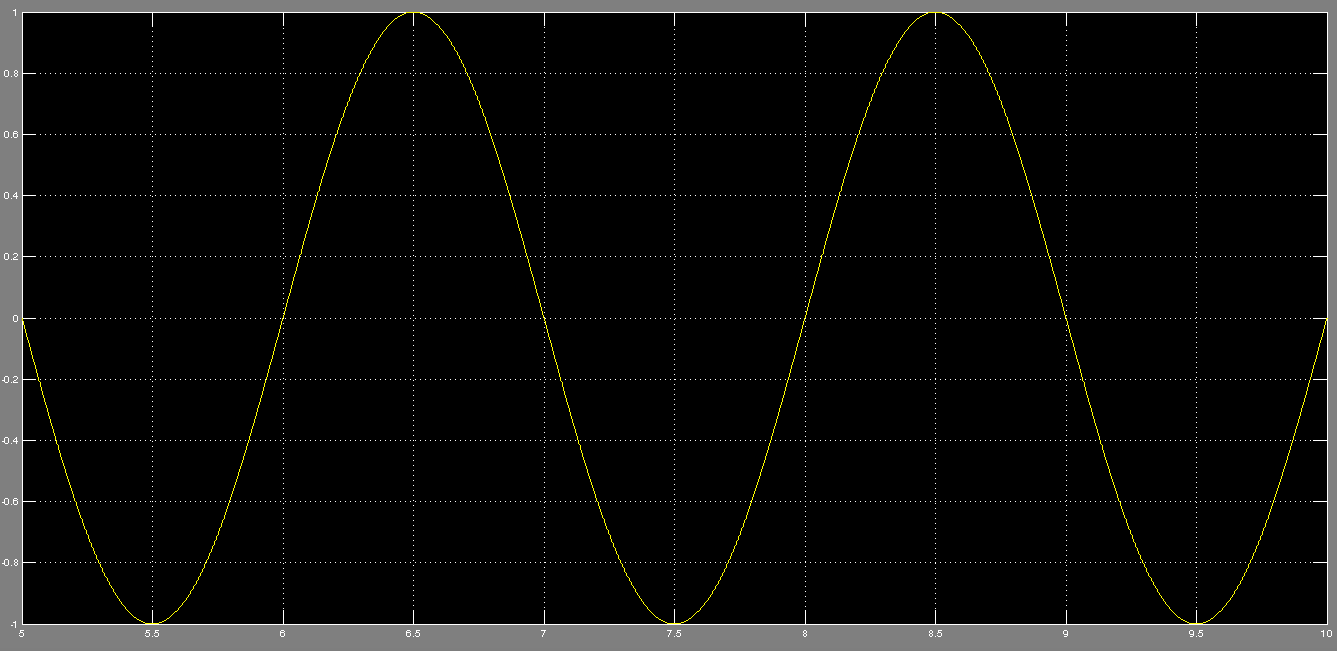
\includegraphics[width=150mm, scale = 0.9]{lab8/8_8}
   \caption{Исходный сигнал}

\end{figure}
\begin{figure}[H]

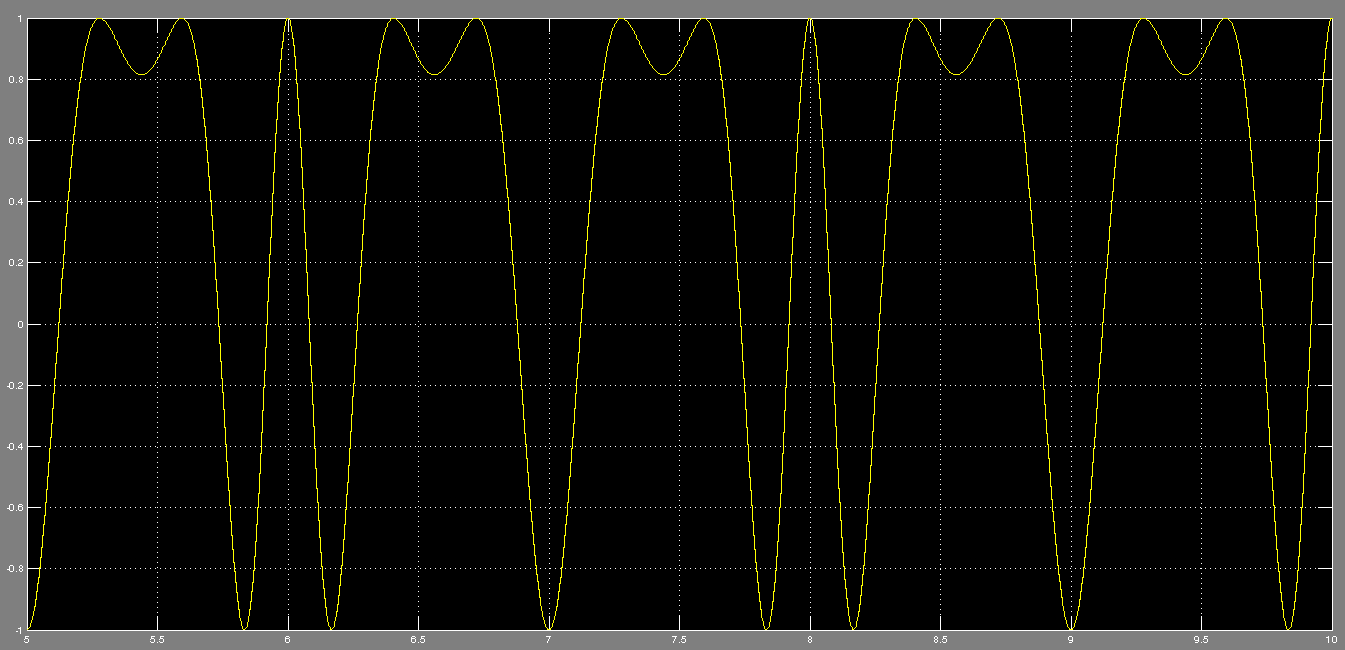
\includegraphics[width=150mm, scale = 0.9]{lab8/8_9}
   \caption{Моделированный сигнал}

\end{figure}
\begin{figure}[H]

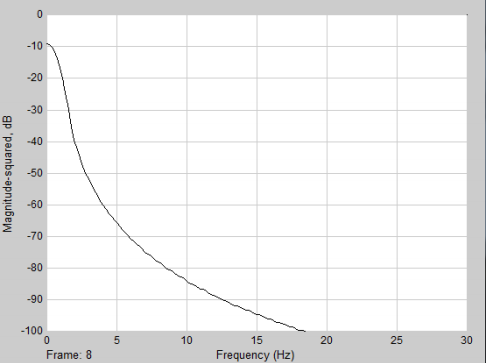
\includegraphics[width=150mm, scale = 0.9]{lab8/8_10}
   \caption{Спектр моделированного сигнала}

\end{figure}
Выполним демодуляцию, в том числе с помощью блока захвата фазы (фазовой автоподстройки частоты) Phase-Locked Loop.
\begin{figure}[H]

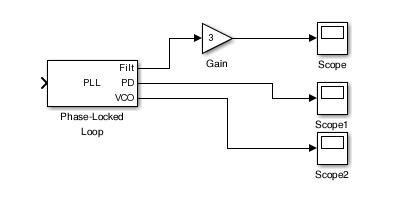
\includegraphics[width=150mm, scale = 0.9]{lab8/8_11}
   \caption{Модель фазовой автоподстройки часоты в режиме слежения}

\end{figure}
\begin{figure}[H]

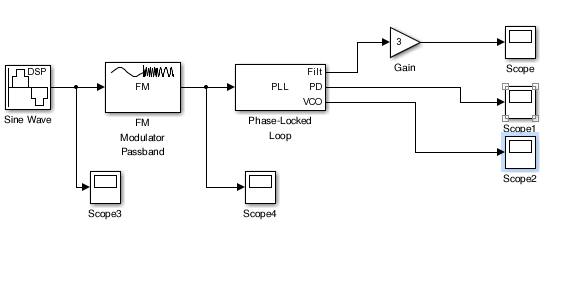
\includegraphics[width=150mm, scale = 0.9]{lab8/8_12}
   \caption{Модель фазовой автоподстройки часоты в режиме захвата и удержания сигнала}

\end{figure}
\begin{figure}[H]

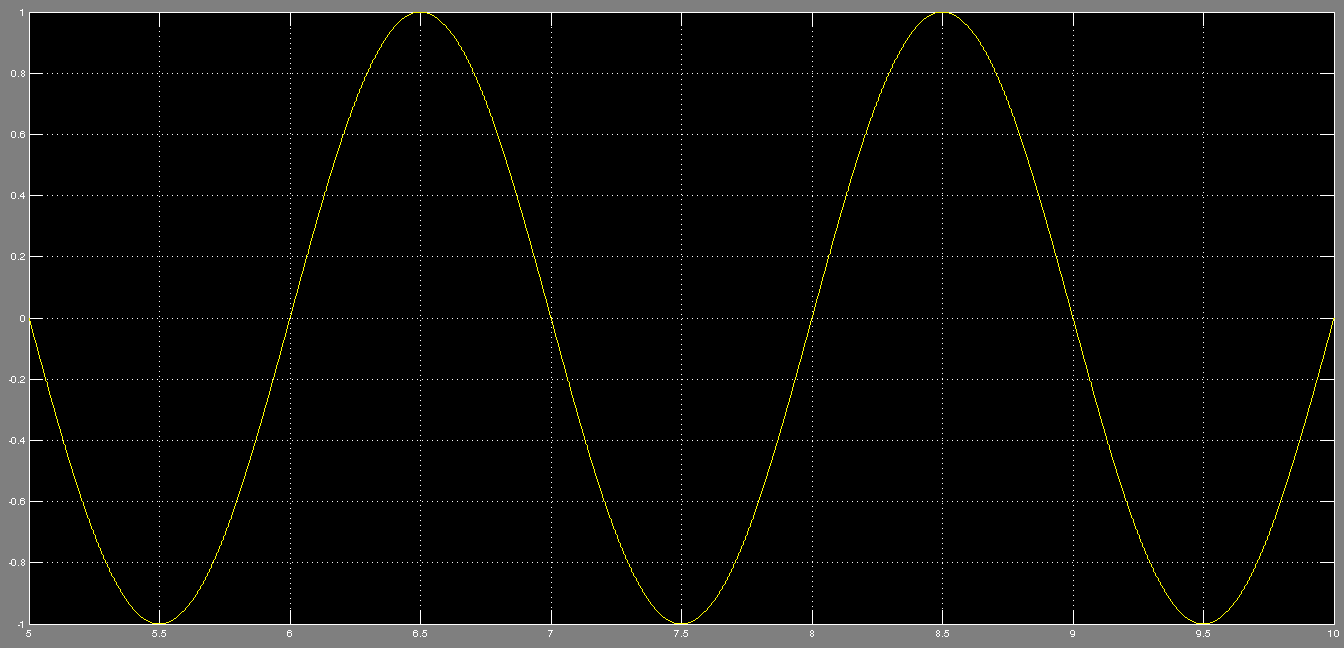
\includegraphics[width=150mm, scale = 0.9]{lab8/8_13}
   \caption{Исходный сигнал}

\end{figure}
\begin{figure}[H]

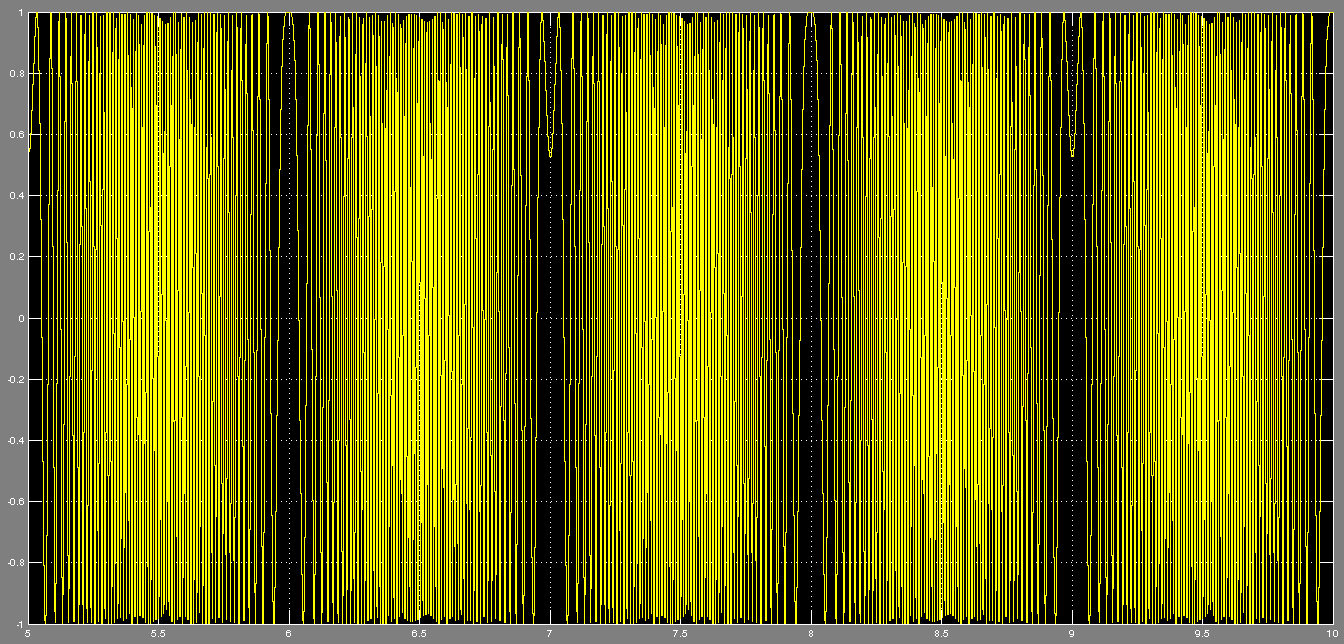
\includegraphics[width=150mm, scale = 0.9]{lab8/8_14}
   \caption{Моделированный сигнал}

\end{figure}
\begin{figure}[H]

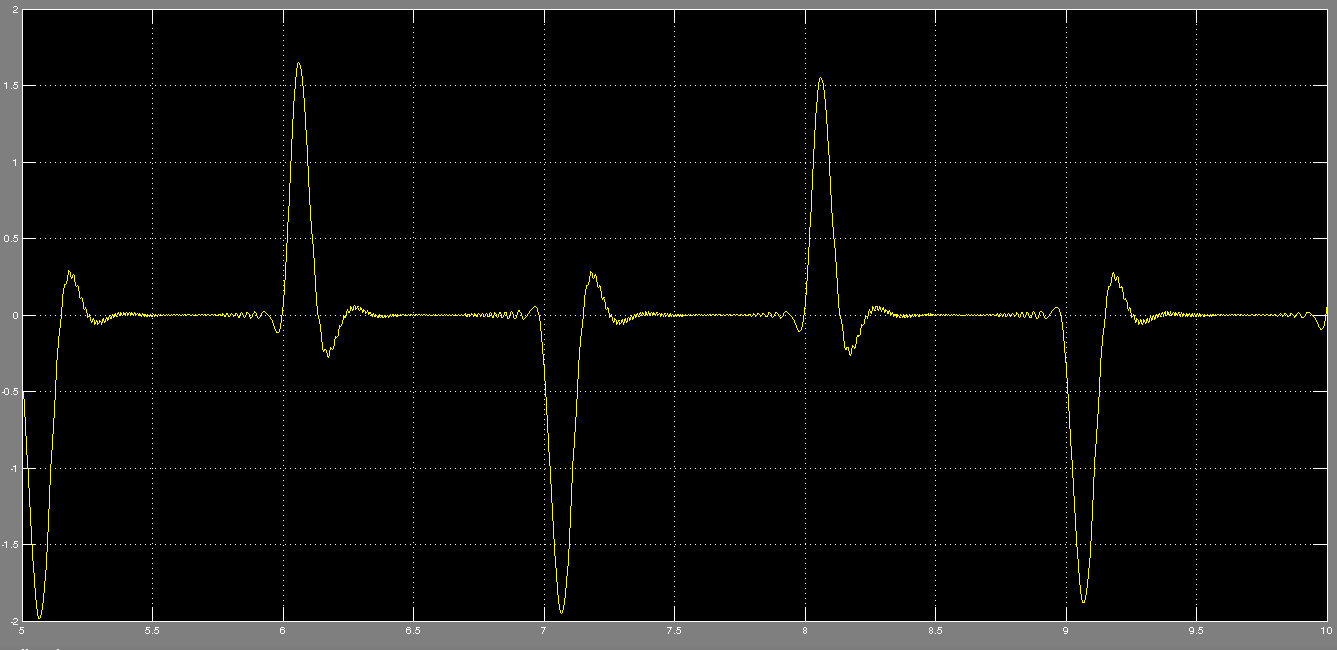
\includegraphics[width=150mm, scale = 0.9]{lab8/8_15}
   \caption{Сигнал на выходе ФНЧ}

\end{figure}
\begin{figure}[H]

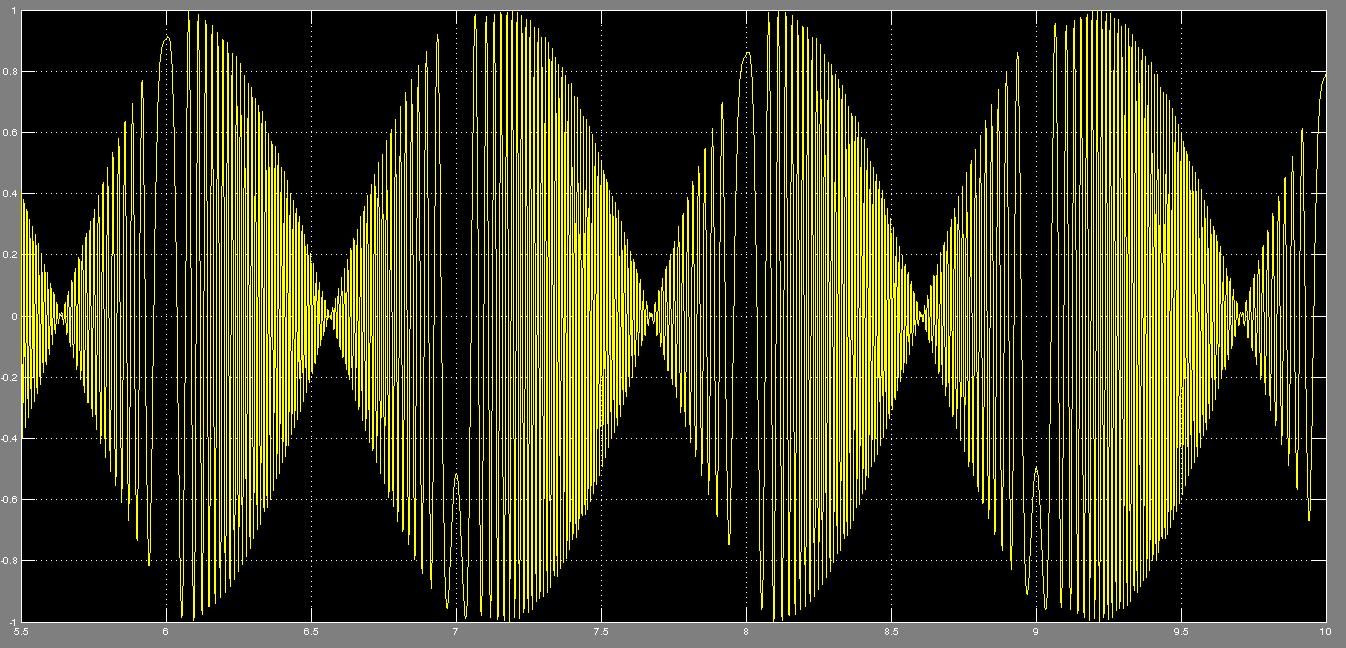
\includegraphics[width=150mm, scale = 0.9]{lab8/8_16}
   \caption{Сигнал на выходе фазового детектора}

\end{figure}
\begin{figure}[H]

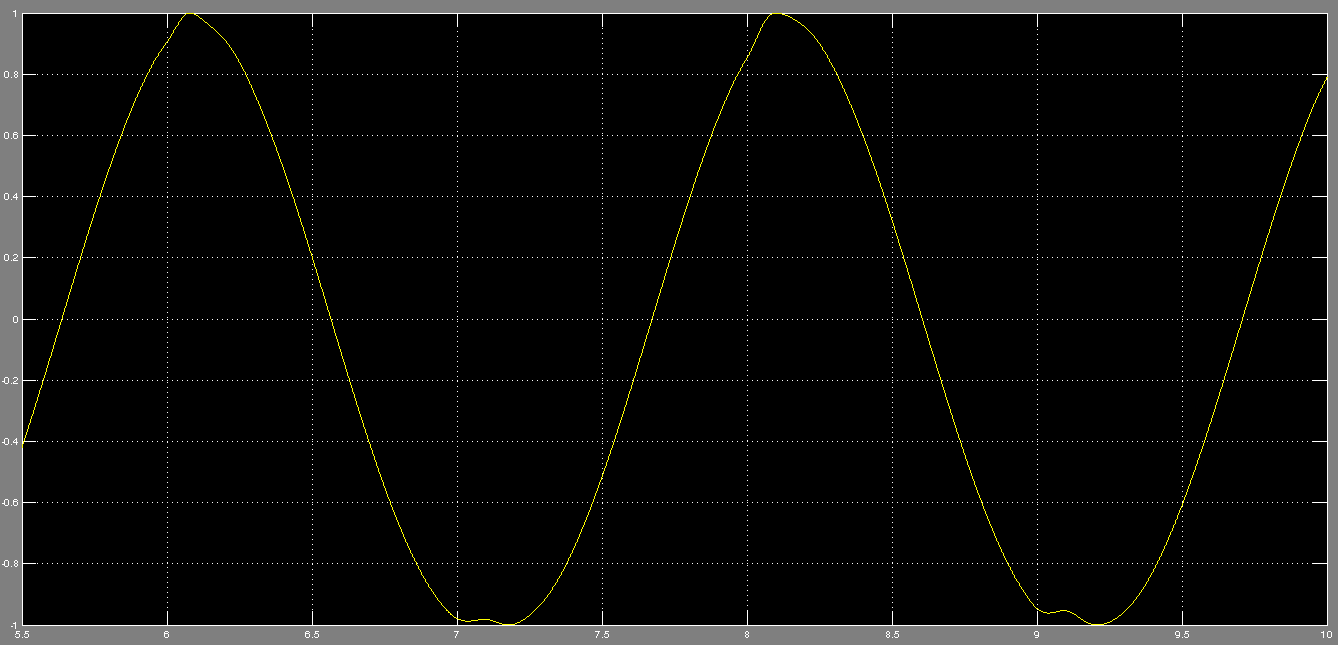
\includegraphics[width=150mm, scale = 0.9]{lab8/8_17}
   \caption{Сигнал на выходе ГУН}

\end{figure}
\section{Вывод}

В результате выполнения данной работы были выполнены частотная и фазовая модуляция/демодуляция, а также чатотная демодуляция с  помощью блока захвата фазы. Частотная и фазовая модуляция тесно взаимосвязаны, поскольку обе они влияют на аргумент функции cos. Поэтому эти два вида модуляции имеют общее название — угловая модуляция. Сигнал с угловой модуляцией имеет вид колебания, начальная фаза которого зависит от времени:
	\begin{equation}
	s_(t) = A_0 cos(\omega0 t + j(t)).
	\end{equation}
%Различие между фазовой и частотной модуляцией заключается лишь в том, как именно начальная фаза $j(t)$ связана с модулирующим сигналом.
В случае фазовой модуляции частота несущей зависит от производной модулируемого сигнала, а в случае частотной - от самого его значения.

Для демодуляции использовалась петля ФАПЧ, состоящая из перемножителя (используемого в качестве фазового детектора), фильтра нижних частот и генератора, управляемого напряжением (ГУН).
% Получаемый на выходе петли ФАПЧ сигнал пропорционален отклонению мгновенной частоты модулированного сигнала от несущей частоты, поэтому при демодуляции ФМ этот сигнал можно дополнительно проинтегрировать, чтобы получить начальную фазу сигнала.